\chapter{Reconstruction}
\label{chap:reconstruction}

Chapter \ref{chap:experiment} discusses how a proton-proton collision may be captured by a physical 
detector and turned into data that may be stored and analyzed. Chapter \ref{chap:simulation} discusses 
the simulation of this same process. At this most basic level, however, the ATLAS detector is only a machine 
for turning particles into a set of electrical signals, albeit in a very sophisticated, physics motivated way. 
This chapter discusses the step of turning these electrical signals into objects which may be identified 
with the underlying physics processes, and therefore used to make statements about what occurred within 
a given collision event. This process is termed \emph{reconstruction}, and we will focus particularly on jets and flavor tagging, as the most relevant pieces for this thesis work.

\section{Jets}
As discussed in Chapters \ref{chap:experiment} and \ref{chap:simulation}, the production of particles with color 
charge from a proton-proton interaction is complicated both by parton showering and by confinement: a quark produced 
from a hard scatter is not seen as a quark, but rather, as a spray of particles with a variety of hadrons in the final 
state, which subsequently shower upon interaction with the calorimeter in a complicated way. 

For hard scatter electrons, photons, or muons on the other hand, the picture is much clearer: there is no parton 
showering, and each has a distinct signature in the detector: photons have no tracks and a very localized calorimeter
shower, electrons are associated with tracks and are similarly localized in the calorimeter, and muons are associated 
with tracks, pass through the calorimeter due to their large mass, and leave signatures in the muon spectrometer.

Jets are a tool to deal with the messiness of quarks and gluons. The basic concept is to group the multitude of
particles produced by hadronization into a single object. Such an object then has associated properties, 
including a four-vector, which may be identified with the corresponding initial state particle. In practice a variety 
of information from the ATLAS detector is used for such a reconstruction. The analysis considered in this thesis uses 
particle flow jets~\cite{PERF-2015-09}, which combines information from both the tracker and the calorimeter, where the 
combined objects may be identified with underlying particles. However, jets built from clusters of calorimeter cells~\cite{PERF-2014-07} as well as from charged particle tracks~\cite{ATL-PHYS-PUB-2017-010} have also been used very effectively.

A variety of algorithms are used to associate detector level objects to a given jet. The most commonly used 
in ATLAS is the anti-$k_{T}$ algorithm~\cite{Antikt}, which is a successor to the $k_{T}$ algorithm, among others~\cite{Jetography}, and develops as follows. Both algorithms are sequential recombination algorithms, which begin with the smallest distance, $d_{ij}$ between considered objects (e.g. particles or intermediate groupings of particles). If $d_{ij}$
is less than a parameter $d_{iB}$ (B for ``beam'') object $i$ is combined with object $j$, the distance $d_{ij}$ is recomputed, and the process repeats. This proceeds until $d_{ij} \geq d_{iB}$, at which point the jet is ``complete''
and removed from the list of considered objects.

The definitional difference between $k_{T}$ and anti-$k_{T}$ is these distance parameters. In 
general form, these are defined as 
\begin{align}
d_{ij} &= \min(p_{Ti}^{2p},p_{Tj}^{2p})\frac{\Delta R_{ij}^2}{R^2}\\
d_{iB} &= p_{Ti}^{2p}
\end{align}
where $p_{Ti}$ is the transverse momentum of object $i$, $\Delta R_{ij}$ is the angular distance between 
objects $i$ and $j$, $R$ is a radius parameter, and $p$ controls the tradeoff between the $p_{T}$ and angular 
distance terms. For the $k_{T}$ algorithm $p=1$; for the anti-$k_{T}$ algorithm, $p=-1$. This is a simple 
change, but results in significantly different behavior. 

The anti-$k_{T}$ algorithm can be understood as follows: for a single high $p_{T}$ particle ($p_{T1}$) 
surrounded by a bunch of low $p_{T}$ particles, the low $p_{T}$ particles will be clustered with the high $p_{T}$ one if
\begin{align}
&d_{1j} = \frac{1}{p_{T1}^2}\frac{\Delta R_{1j}^2}{R^2} < \frac{1}{p_{T1}^2}\\
&\implies \Delta R_{1j} < R.
\end{align}
Therefore, a single high $p_{T}$ particle ($p_{T1}$) surrounded by a bunch of low $p_{T}$ particles results 
in a perfectly conical jet. This shape may change with the presence of other high momentum particles, but the
key feature of the dynamics is that the jet shape is determined by high $p_{T}$ objects due to the $\frac{1}{p_{T}}$
nature of this definition. In contrast, the $k_{T}$ algorithm results in jets influenced by low momentum particles, 
which results in a less regular shape. This property, of regular jet shapes determined by high momentum objects, 
as well as demonstrated good practical performance, makes the anti-$k_{T}$ algorithm the favored jet algorithm in ATLAS.

Because jets are composed of multiple objects, a useful property of jets is jet \emph{substructure}, that is, 
acknowledging that jets are composite objects, analyzing the structure of a given jet to infer physics information. 
This leads to the use of \emph{subjets}; that is, after running jet clustering, often to create a``large-R'', $R=1.0$ 
anti-$k_{T}$ jet, a smaller radius jet clustering algorithm is run within the jet. Subjets are often chosen using the 
$k_{T}$ algorithm, which again is sensitive to lower momentum particles, with $R=0.2$ or 0.3. For the boosted version 
of this thesis analysis, such a strategy is used, in which the subjets are \emph{variable radius} and depend on the 
momentum of the (proto)jet in question. Beyond this thesis work, substructure is used in a large variety of analyses, 
with a set of associated variables and tools developed for exploiting this structure \todo{Cite some?}.
 
\section{Flavor Tagging}
For this this thesis, the physics process being considered is $HH\rightarrow \bbbb$. From the previous section, we 
know that the standard practice is to identify these $b$ quarks (or, rather, the resulting $B$ hadrons, due to confinement) 
with jets -- in our case, these \emph{$b$-jets} are R=0.4 anti-$k_{T}$ particle flow jets (see Chapter \ref{chap:bbbb}). 
However, not all jets produced at the LHC are from $B$ hadrons; rather, there are a variety of different types of jets 
corresponding to different flavors of quarks. These are often classified as light jets (from $u$, $d$, or $s$ quarks, or 
gluons) or as other \emph{heavy flavor} jets, e.g. $c$-jets, involving $c$ quarks. Distinguishing between these different 
categories is a very active area of work in ATLAS, termed \emph{flavor tagging}, with much focus on \emph{$b$-tagging} in 
particular, that is, the identification of jets from $B$ hadron decays. We here briefly describe the techniques used 
for flavor tagging in ATLAS.

What distinguishes a $b$-jet from any other jet? This question is fundamental to the design of the various $b$-tagging 
algorithms, and has two major answers: (1) $B$ hadrons have long lifetimes, and (2) $B$ hadrons have large masses. 
It is most illustrative to compare the $B$ hadron properties to a common light meson, e.g. $\pi^{0}$, the neutral 
pion, with quark content $\frac{1}{\sqrt{2}}(u\bar{u}-d\bar{d})$. $B$ hadrons have lifetimes around \SI{1.5}{\ps},
corresponding to a decay length $c\tau\approx 0.45$mm. In contrast, $\pi^0$ has a lifetime of $8.4\times 10^{-5}$ps, 
which is around 20,000 times shorter! Theoretically, this comes from CKM suppression of the $b$ to $c$ transition, which dominates the $B$ decay modes. Experimentally, this difference pops up as shown in 
Figure \ref{fig:bjet-diagram} -- light flavor initiated jets decay almost immediately at the proton-proton 
interaction point, whereas b-jets are distinguished by a displaced secondary vertex, corresponding to the 5 mm decay 
length calculated above. This displaced vertex falls short of the detector itself, but may be inferred from larger 
transverse (perpendicular to beam) and longitudinal (parallel to beam) impact parameters of the resulting tracks, 
termed $d_{0}$ and $z_{0}$ respectively.

\begin{figure}[ht]
\centering
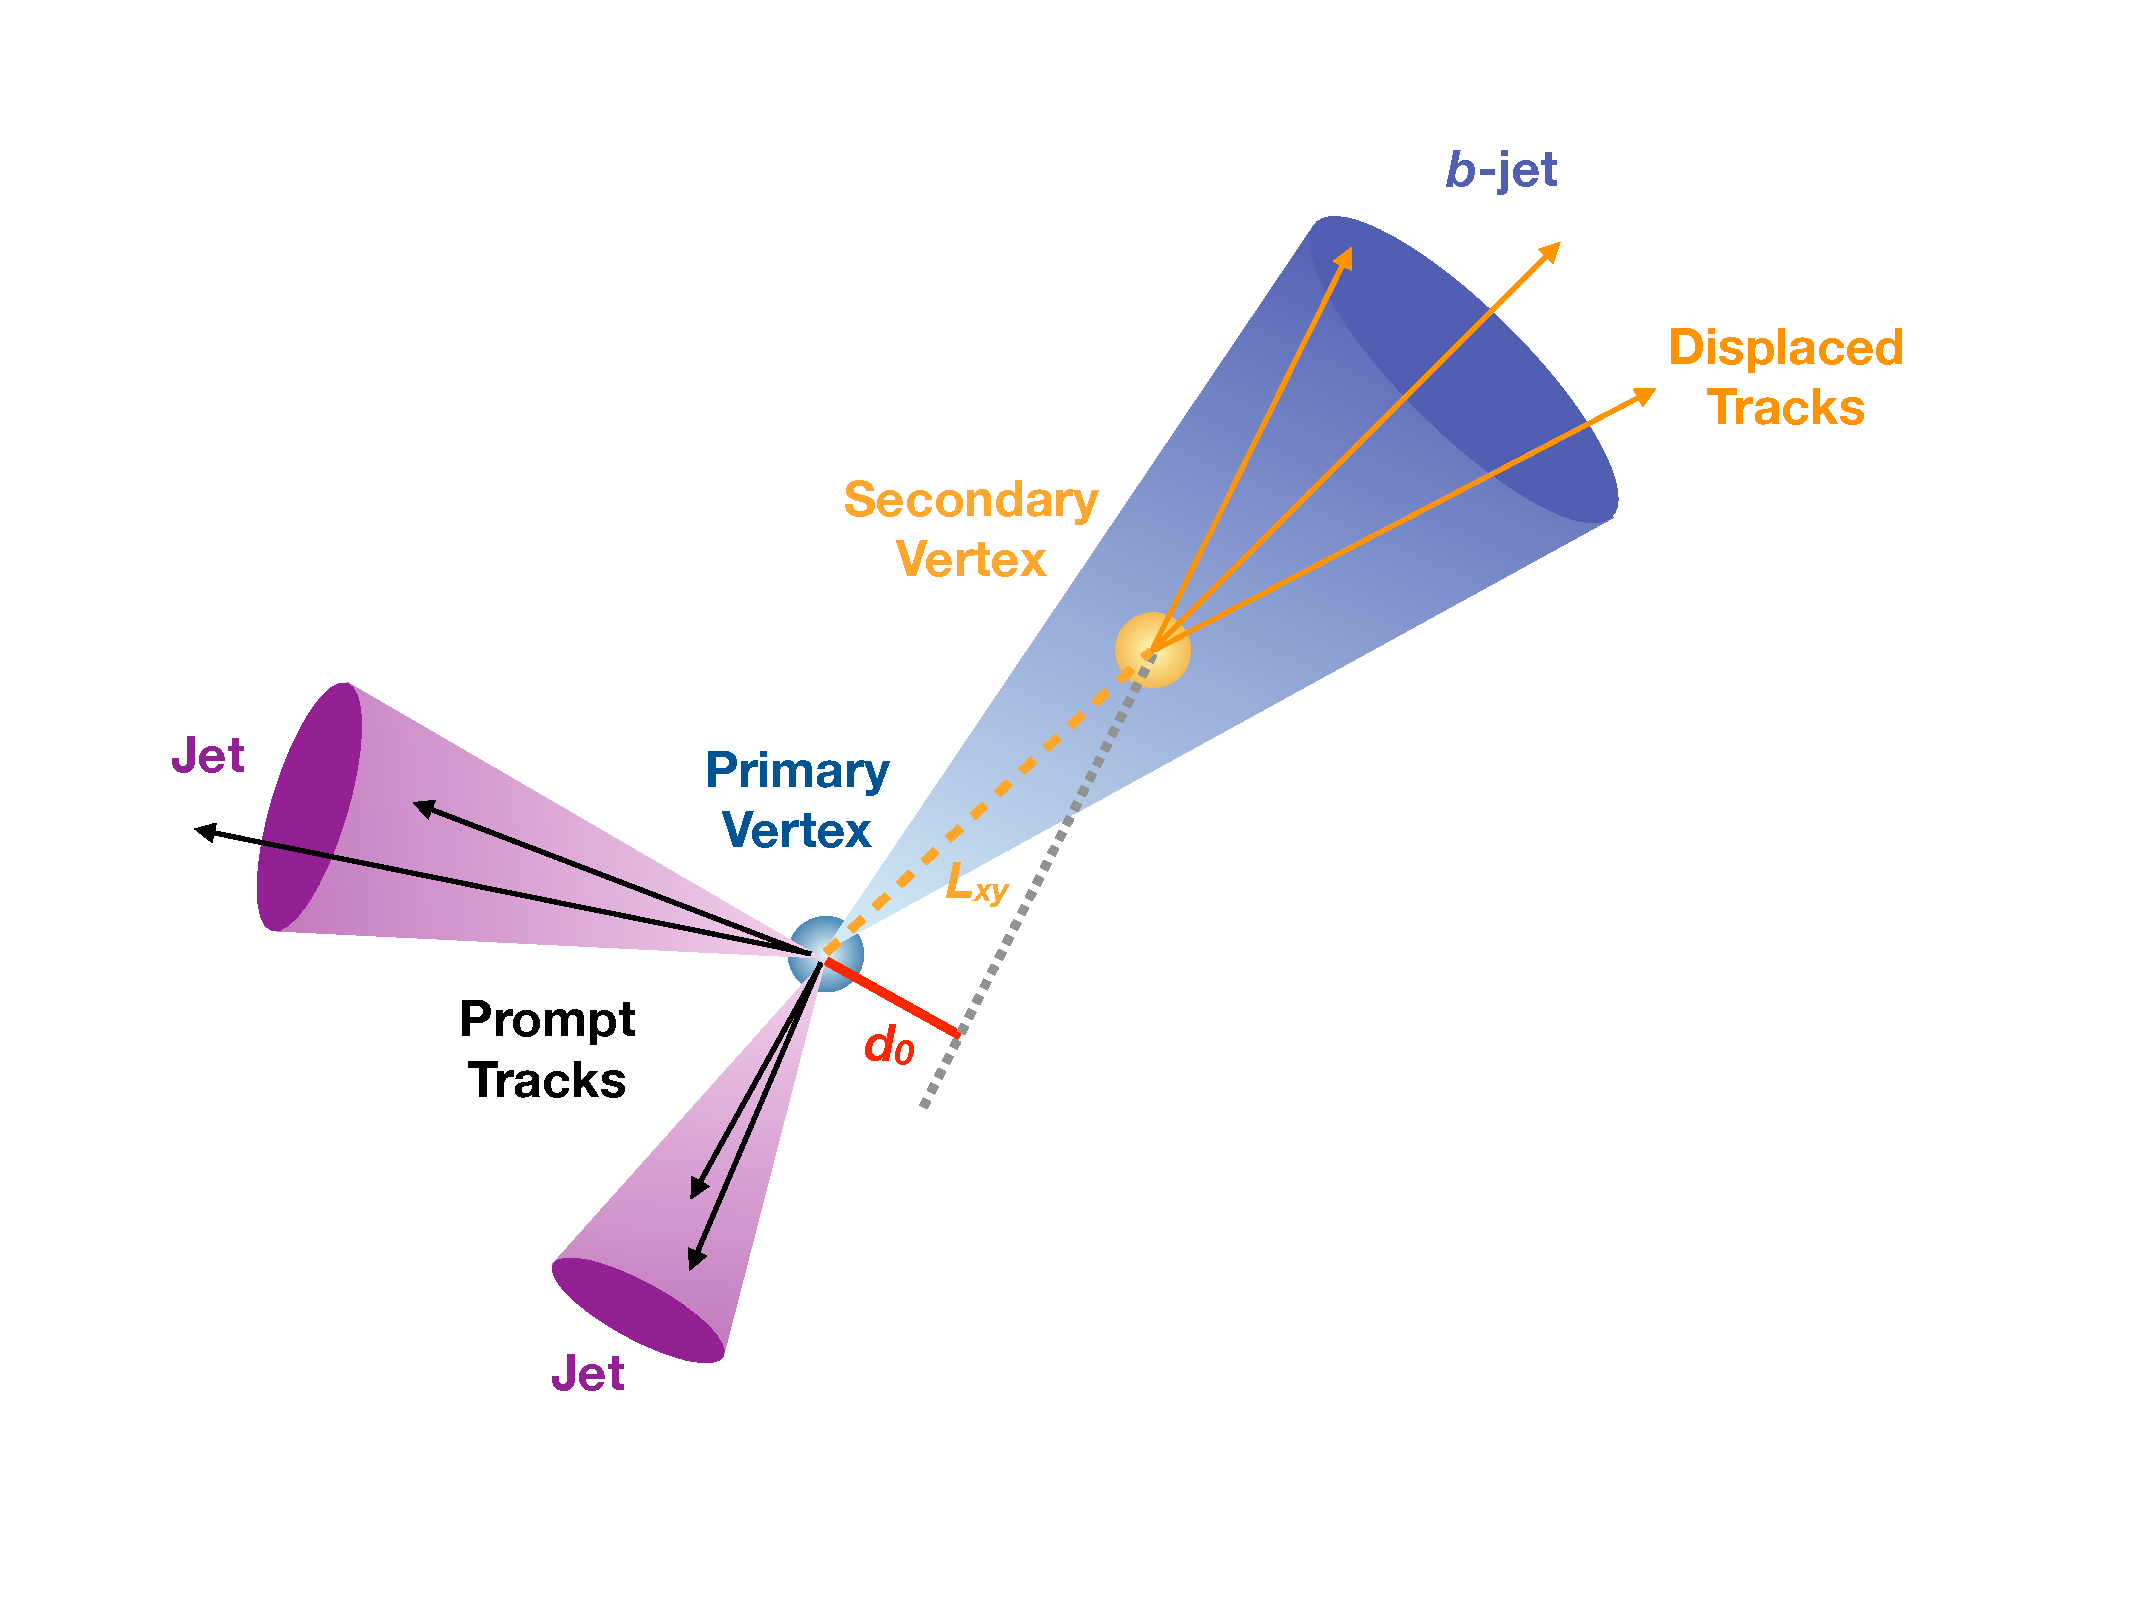
\includegraphics[width=0.8\textwidth]{figures/bjet-diagram.pdf}
\caption{\label{fig:bjet-diagram} Illustration of an interaction producing two light jets and one $b$-jet 
in the transverse plane. While the light jets decay ``promptly'', coinciding with the primary vertex of the 
proton-proton interaction, the longer lifetime of $B$ hadrons leads to a secondary decay vertex, displaced from 
the primary vertex by length $L_{xy}$. This is typically a few mm, and therefore is not directly visible in the 
detector, but leads to a large transverse impact parameter, $d_{0}$, for the resulting tracks.~\cite{bjettrigger}}
\end{figure}

Coming to the mass, $B$ mesons have masses of around \SI{5.2}{\GeV}, whereas the $\pi^{0}$ mass is around \SI{0.134}{\GeV},
(around 40 times lighter). This higher mass gives access to a larger decay phase space, leading to a high multiplicity 
for $b$-jets (average of 5 charged particles per decay).

One final distinguishing feature of $B$ hadrons is their \emph{fragmentation function}, a function describing the 
production of an observed final state. For $B$ hadrons, this is particularly ``hard'', with the $B$ hadrons themselves 
contributing to an average of around 75~\% of the $b$-jet energy. Thus, the identification of $b$-jets with $B$ hadrons 
is, in some sense, descriptive.

We have contrasted $b$-jets and light jets, demonstrating that there are several handles available for making this 
distinction. $c$-jets are slightly more similar to $b$-jets, but the same handles still apply -- $c$-hadron lifetimes are
between \SIlist{0.5;1}{\ps}, a factor of 2 smaller than $B$ hadrons. Their mass is around \SI{1.9}{\GeV}, 2 to 3 times 
smaller than $B$ hadrons, and $c$-hadrons contribute to an average of around 55~\% of $c$-jet energy. Therefore, while 
the gap is slightly smaller, a distinction may still be made.

The ATLAS flavor tagging framework~\cite{FTAG-2018-01} relies on developing a suite of ``low-level'' taggers, which 
use a variety of information about tracks and vertices as inputs. The output of these lower level taggers are then 
fed into a higher level tagger, which aggregates these results into a high level discriminant. Each of these taggers 
is described below.

\FloatBarrier
\subsection{IP2D/3D}
IP2D and IP3D are taggers based on the large track impact parameter (IP) nature of $B$ hadron decays. Both are 
based on histogram templates derived from Monte Carlo simulation, which are used as probability density 
functions to construct log-likelihood discriminants. IP2D incorporates just the transverse impact parameter 
information using 1D histogram templates, whereas IP3D uses both transverse and longitudinal impact parameters 
in a 2D template, which accounts for correlations. Importantly, these are \emph{signed} impact 
parameters, with sign based on the angle between the impact parameter and the considered jet -- positive impact 
parameters are consistent with a track extrapolation in front of the jet (angle between impact parameter 
line and jet $<90^{\circ}$), and therefore more consistent with tracks originating from a displaced decay.

Rather than using the impact parameters directly, an impact parameter \emph{significance} is used which 
incorporates an uncertainty on the impact parameter -- tracks with a lower uncertainty but the same impact 
parameter will contribute more in the calculation. This signed significance is what is used to sample from the 
PDF templates, with the resulting discriminants the sum of probability ratios between given jet hypotheses over 
tracks associated to a given jet, namely $\sum_{i=1}^{N} \log{\frac{p_{b}}{p_{light}}}$ between $b$-jet and 
light jet hypotheses, where $p_{b}$ and $p_{light}$ are the per-track probabilities. Similar discriminants 
are defined between $b$- and $c$-jets and $c$ and light jets. \todo{show distributions?}

\subsection{SV1}
SV1 is an algorithm which aims to find a secondary vertex (SV) in a given jet. Operating on all 
vertices associated with a considered jet, the algorithm discards tracks based on a variety of cleaning 
requirements. It then proceeds to first construct all two-track vertices, and then iterates over all the 
tracks involved in these two track vertices to try to fit a single secondary vertex, which would then be 
identified with the secondary vertex from the $b$ or $c$ hadron decay. This fit proceeds by evaluating 
a $\chi^2$ for the association of a track and vertex, removing the track with the largest $\chi^2$, 
and iterating until the $\chi^2$ is acceptable and the vertex has an invariant mass of less than 
\SI{6}{\GeV} (for consistency with $b$ or $c$ hadron decay).

A variety of discriminating variables may then be constructed, including (1) invariant mass of the secondary 
vertex, (2) number of tracks associated with the secondary vertex, (3) number of two-track vertices, 
(4) energy fraction of the tracks associated to the secondary vertex (relative to all of the tracks 
associated to the jet), and various metrics associated with the secondary vertex position and decay length, 
including (5) transverse distance between the primary and secondary vertex, (6) distance between the primary 
and secondary vertex (7) distance between the primary and secondary vertex divided by its uncertainty, 
and (8) $\Delta R$ between the jet axis and the direction of the secondary vertex relative to the primary
vertex.

While all eight of these variables are used as inputs to the higher level taggers, the number of two-track vertices, 
the vertex mass, and the vertex energy fraction are additionally used with 3D histogram templates to evaluate 
flavor tagging performance by constructing log-likelihood discriminants, similar to the procedure for 
IP2D/3D.

\subsection{JetFitter}
Rather than focusing on a particular aspect of the $B$ hadron or $D$ hadron decay topology (e.g impact parameter 
or secondary vertex), the third low level tagger, \textsc{JetFitter}\xspace~\cite{ATL-PHYS-PUB-2018-025}, 
tries to reconstruct the full decay chain, including all involved vertices. This is structured around a 
Kalman filter formalism~\cite{Kalman}, and has the strong underlying assumption that all tracks which stem 
from $B$ and $D$ hadron decay must intersect a common flight path. This assumption provides significant constraints, 
allowing for the reconstruction of vertices from even a single track, reducing the number of degrees of 
freedom in the fit, and allowing the use of ``downstream'' information, e.g., compatibility of tracks with 
a $B\rightarrow D$-like decay. The constructed topology, including primary vertex location and $B$-hadron flight 
path, is iteratively updated over tracks associated to a given jet, and a variety of discriminating variables 
related to the resulting topology and reconstructed decay are used as inputs to the high level taggers.

\subsection{RNNIP}
The IP2D and IP3D algorithms rely on per-track probabilities, and the final discriminating variables (and inputs 
to the higher level taggers) are sums (products) over these independently considered quantities. In practice, 
however, the tracks are not independent -- this is merely a simplifying assumption to allow for the use of a 
binned likelihood, as treatment of all of the interdependencies in such a framework quickly becomes intractable. 
To address this issue, a recurrent neural network-based algorithm, RNNIP~\cite{ATL-PHYS-PUB-2017-003}, is used, 
which takes as input a variety of per-track variables, including the signed impact parameter significances (as in 
IP3D) as well as track momentum fraction relative to the jet and $\Delta R$ between the track and the jet. RNNs 
are sequence-based, and vectors of input variables corresponding to tracks for a given jet are ordered by magnitude of 
transverse impact parameter significance and then passed to the network, which outputs class probabilities corresponding 
to b-jet, c-jet, light-jet, and $\tau$-jet hypotheses. Such a procedure allows the network to learn interdependencies between tracks, improving performance.

\subsection{MV2 and DL1}
Outputs from the above taggers are combined into high level taggers to aggregate all of the information and 
improve discriminating power relative to the respective individual taggers as, as shown in Figure 
\ref{fig:low-vs-high-tag}. These high level taggers are primarily in two forms: MV2, which uses a Boosted 
Decision Tree (BDT) for this aggregation, and DL1, which uses a deep neural network. For the baseline versions of 
these taggers, only inputs from IP2D, IP3D, SV1, and JetFitter are used. The tagger used for this thesis analysis, 
DL1r, additionally incorporates RNNIP, demonstrating improved performance over the baseline DL1, as shown in 
Figure \ref{fig:DL1-vs-DL1r}. All high level taggers also include jet $p_{T}$ and $|\eta|$.

DL1 offers a variety of improvements over MV2. Rather than a single discriminant output, 
as with MV2, DL1 has a multidimensional output, corresponding to probabilities for a jet to be a $b$-jet, $c$-jet, 
or light jet. This allows the trained network to be used for both $b$- and $c$-jet tagging. The final discriminant 
for $b$-tagging with DL1 correspondingly takes the form
\begin{equation}
D_{\text{DL1}} = \ln{\qty(\frac{p_{b}}{f_{c}\cdot p_c+(1-f_c)\cdot p_{\text{light}}})}
\end{equation}
where $p_b$, $p_c$, and $p_{light}$ are the output $b$, $c$, and light jet probabilities, and $f_{c}$
corresponds to an effective $c$-jet fraction, which may tuned to optimize performance.

DL1 further includes an additional set of \textsc{JetFitter}\xspace input variables relative to MV2 
which correspond to $c$-tagging -- notably properties of secondary and tertiary vertices, as would be 
seen in a $B\rightarrow D$ decay chain. 

\begin{figure}[ht]
\centering
\subfloat{
	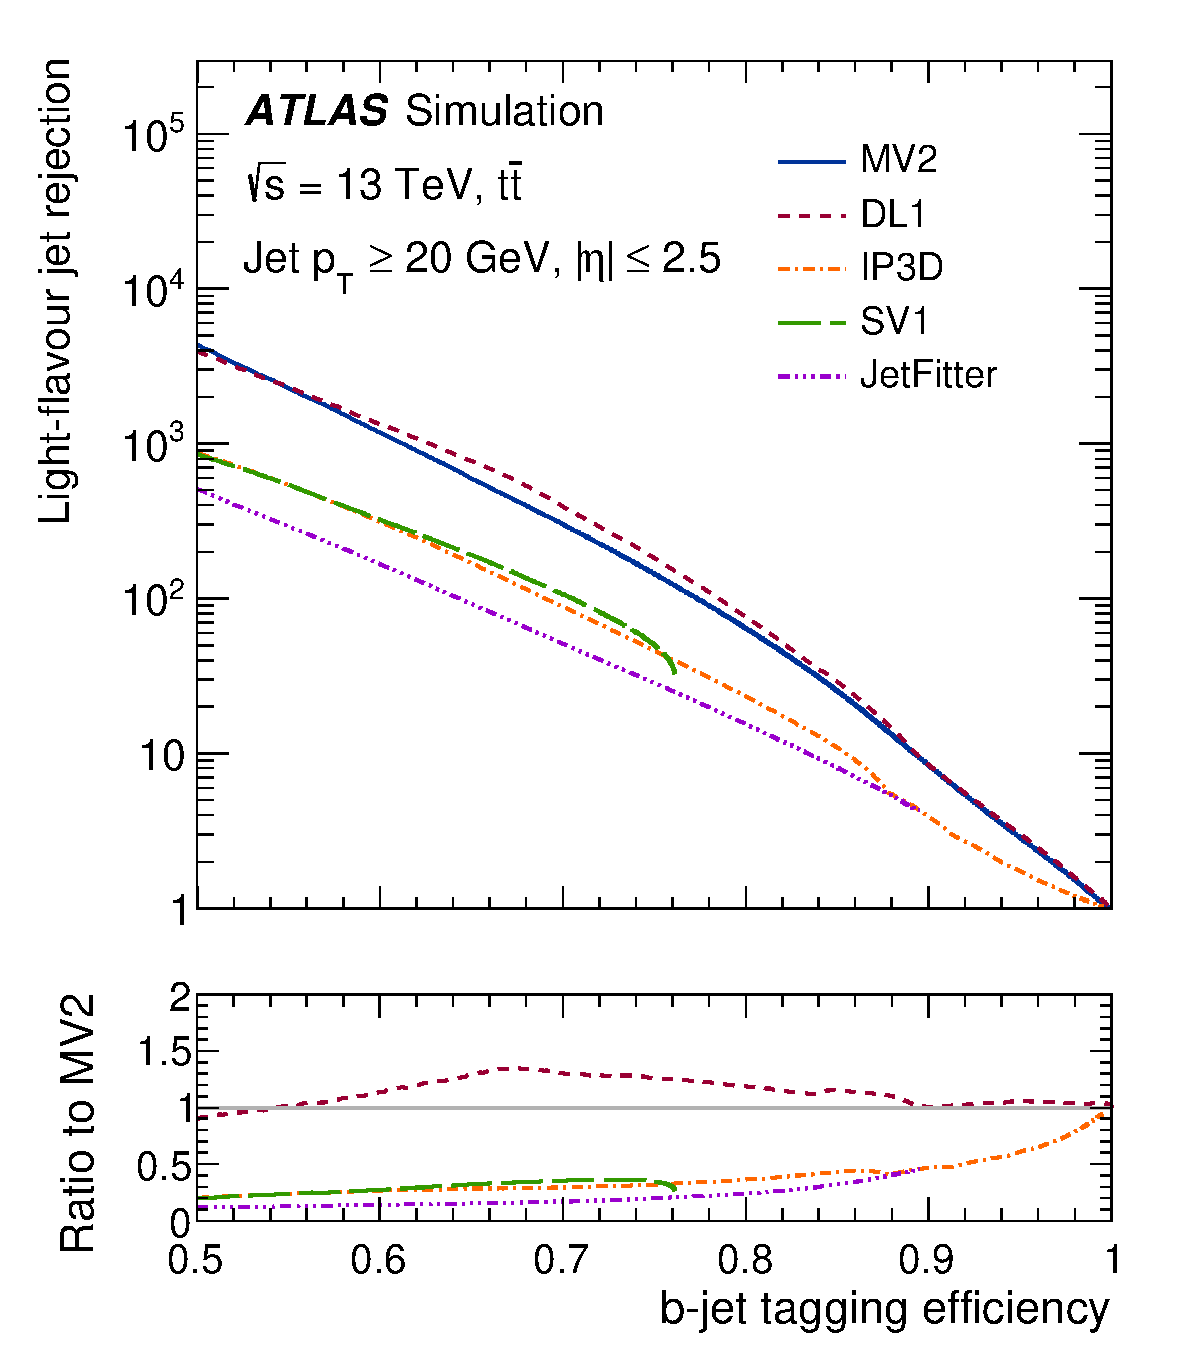
\includegraphics[width=0.48\textwidth]{figures/DL1-vs-low-level-light-jet.pdf}
}
\subfloat{
	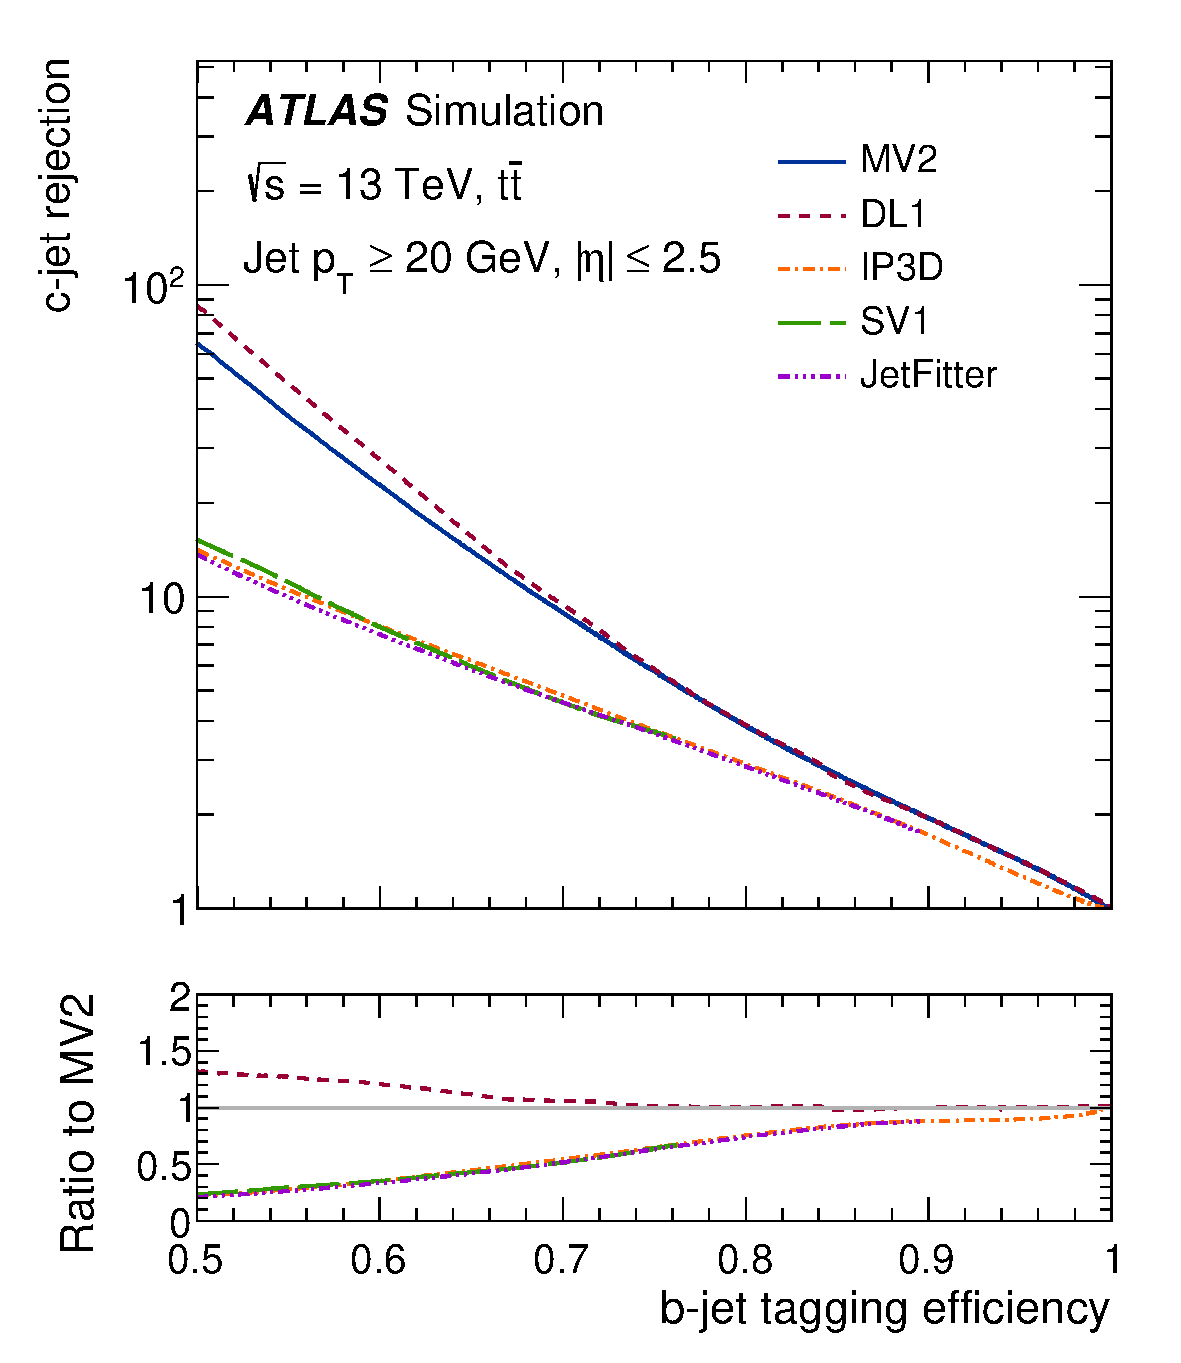
\includegraphics[width=0.48\textwidth]{figures/DL1-vs-low-level-c-jet.pdf}
}
\caption{\label{fig:low-vs-high-tag} Performance of the various low and high level flavor tagging algorithms 
in $t\bar{t}$ simulation, demonstrating the tradeoff between $b$-jet efficiency and light and $c$-jet rejection. 
The high level taggers demonstrate significantly better performance than any of the individual low level 
taggers, with DL1 offering slight improvements over MV2 due to the inclusion of additional input variables.}
\end{figure}


Figure \ref{fig:low-vs-high-tag} shows a comparison of the performance of the various taggers. 
The $b$-tagging performance of DL1 and MV2 is found to be similar, with some improvements in 
light jet and $c$-jet rejection from the additional variables used in DL1. 
The performance of these high level taggers additionally is seen to be significantly better than any of the 
individual low level ones, even in regimes where only a single low level tagger is relevant (such as high 
b-tagging efficiencies, where SV1 and \textsc{JetFitter}\xspace are limited by selections on tracks 
entering the respective algorithms).

The inclusion of RNNIP offers a significant improvement on top of baseline DL1, as shown in Figure 
\ref{fig:DL1-vs-DL1r}, strongly motivating the choice of DL1r for this thesis. 

\begin{figure}[ht]
\centering
\subfloat{
	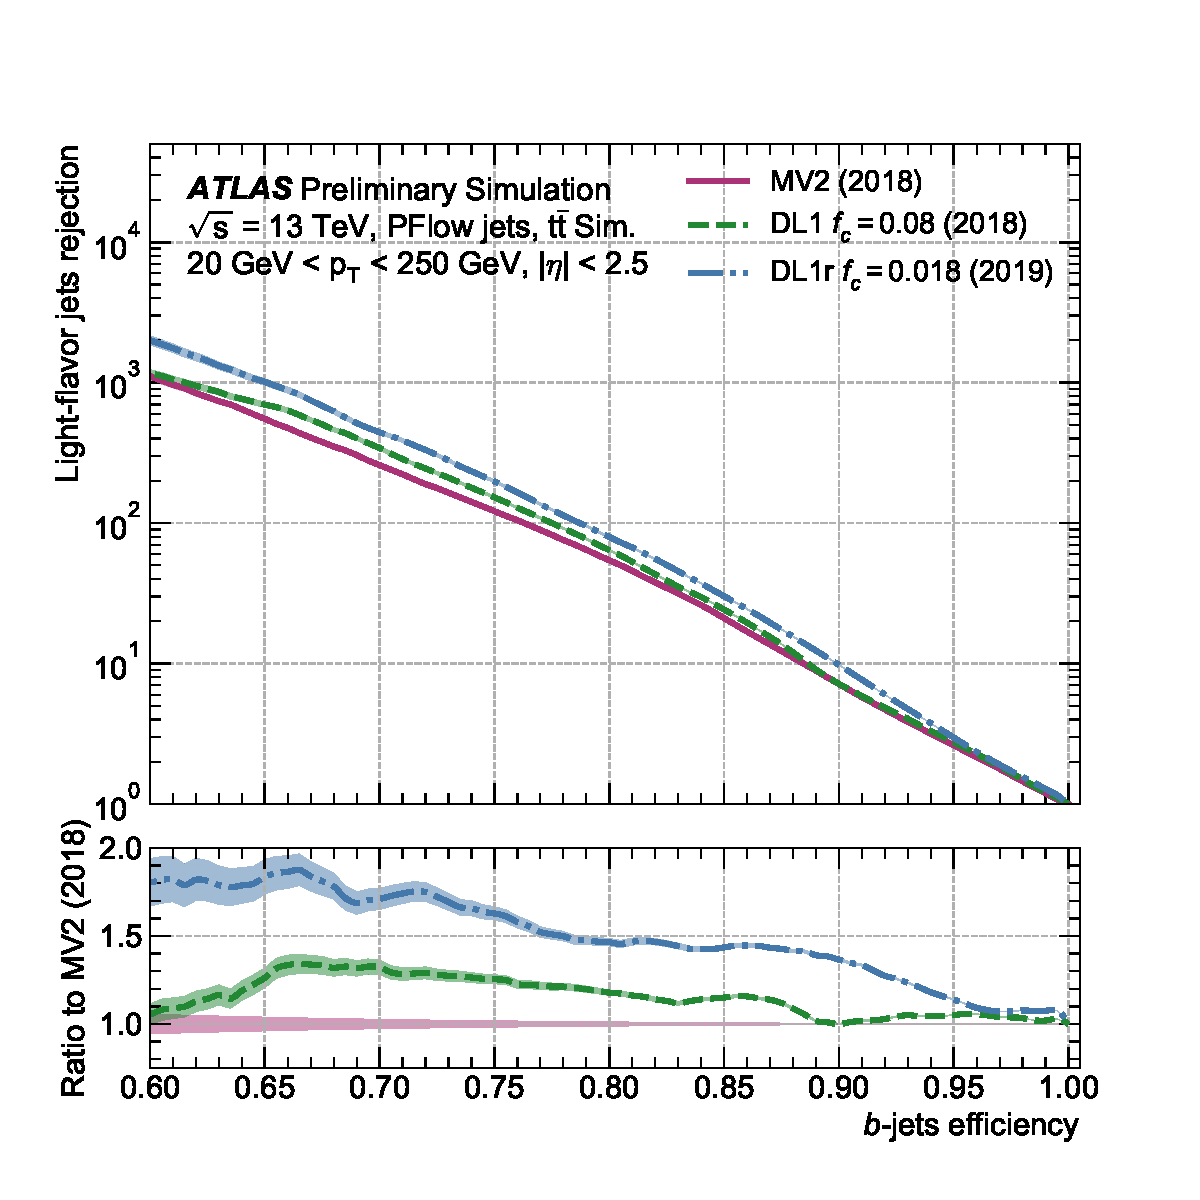
\includegraphics[width=0.48\textwidth]{figures/pflow-DL1-DL1r-light-jet.pdf}
}
\subfloat{
	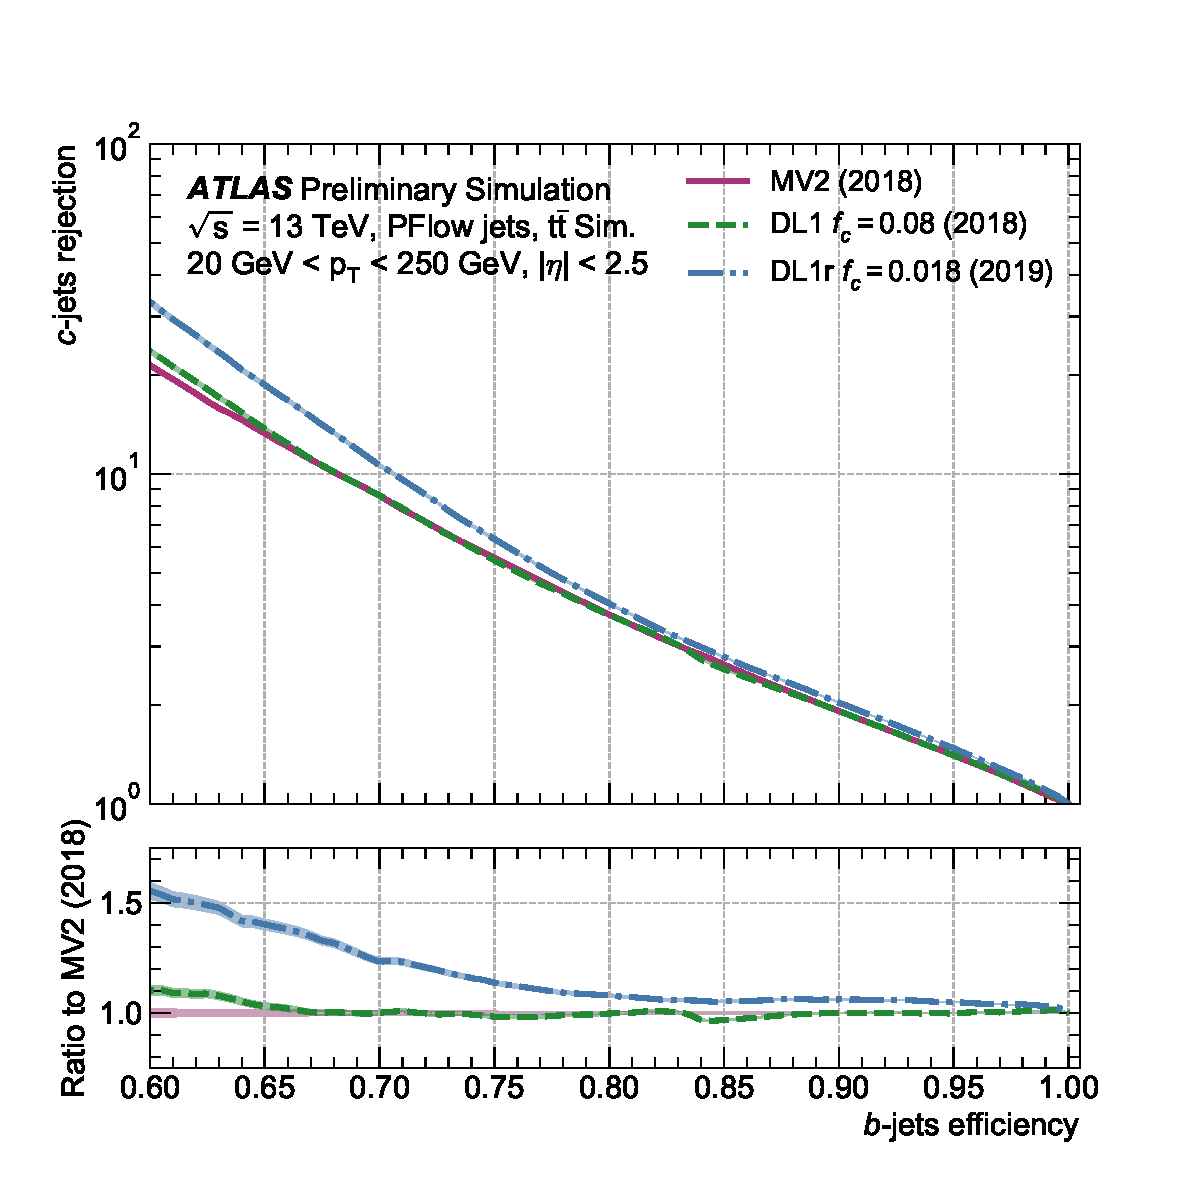
\includegraphics[width=0.48\textwidth]{figures/pflow-DL1-DL1r-c-jet.pdf}
}
\caption{\label{fig:DL1-vs-DL1r} Performance of the MV2, DL1, and DL1r algorithms in $t\bar{t}$ simulation, 
demonstrating the tradeoff between $b$-jet efficiency and light and $c$-jet rejection. $f_{c}$ controls the 
importance of $c$-jet rejection in the discriminating variable, and values shown have been optimized separately 
for each DL1 configuration. DL1r demonstrates a significant improvement in both light and $c$ jet rejection over 
MV2 and DL1.~\cite{PFlowPublicPlots2019}}
\end{figure}


\subsection{Some Practical Notes}
The $b$-tagging metrics presented in Figures \ref{fig:low-vs-high-tag} and \ref{fig:DL1-vs-DL1r} correspond 
to evaluating a tradeoff between $b$-jet efficiency and light jet and $c$-jet rejection. In this case, $b$-jet 
efficiency is defined such that, e.g. for a 77~\% efficiency, 77~\% of the real $b$-jets will be tagged 
as such. Somewhat counterintuitively, this means that a lower $b$-jet efficiency corresponds 
to a more aggressive (``tighter'') selection on the discriminating variable, while a higher 
$b$-jet efficiency corresponds to a less aggressive (``looser'') cut (100~\% efficiency means 
no cut). Light and $c$ jet efficiencies are defined similarly, with rejection defined as $1 /$ the 
corresponding efficiency.

In ATLAS, the respective $b$-tagging efficiencies are used to define various $b$-tagging 
working points. The working point used for the nominal $b$-jet identification in this 
thesis is 77~\% with DL1r. A loosened (less aggressive) selection at the 85~\% working point 
is additionally used. See Chapter \ref{chap:bbbb} for further details.

